%% A simple template for a term report using the Hagenberg setup
%% based on the standard LaTeX 'report' class
%% äöüÄÖÜß  <-- no German Umlauts here? Use an UTF-8 compatible editor!

%%% Magic comments for setting the correct parameters in compatible IDEs
% !TeX encoding = utf8
% !TeX program = pdflatex 
% !TeX spellcheck = en_US
% !BIB program = biber

\documentclass[notitlepage,english]{hgbreport}

\RequirePackage[utf8]{inputenc}		% remove when using lualatex oder xelatex!

\graphicspath{{images/}}  % where are the images?
\bibliography{references}  % requires file 'references.bib'

\makeatletter
\renewcommand{\@chapapp}{Assignment}
\makeatother

%%%----------------------------------------------------------
\author{Peter A.\ Wiseguy}
\title{IM520/MC505 Computer Vision\\ % the name of the course or project
			Term Report}
\date{\today}
%%%----------------------------------------------------------
\usepackage{mathtools}

\usepackage[algo2e,ruled,vlined]{algorithm2e} 
\usepackage[section]{placeins}


\DeclarePairedDelimiter{\abs}{\lvert}{\rvert}

%%%----------------------------------------------------------
\begin{document}
%%%----------------------------------------------------------




%%%----------------------------------------------------------
\chapter{Circle detection in binary dot images}
%%%----------------------------------------------------------


\section {Introduction}
The goal of this exercises was to find a points which could form a circle in a black-white image, consisting of random-noise. While the definition of the problem might not sound serious, research for possible solutions carried out.\cite{fourie2017robust} proposes Harmony Search, an optimization method inspired by music.In \cite{alomari2013randomized} authors propose randomized algorithm, incorporating also edge detection.


\section {Approach}

To describe approach which was used to solve the problem, firstly some notation should be stated. A point in a 2 dimensional space is defined as follows:
\[p_{i}=(u_{i},k_{i})\]
where \i is an index of i-th point
Equation of a circle is defined as follows:
\[(x-x_{i})^2+(y-y_{i})^2=r^2\]
where \i is an index of i-th point


The algorithm is based on collecting all of the points (that is to say, checking which pixel of an image is black, when we operate on white background or white, when the colors are reversed). In the next step random sample of three points is performed. Having three points selected,  it is possible to obtain circle equation. Basing on \cite{wiki:Circles} and high school mathematics materials available in the internet, such as \cite{eisle}, following equations are obtained:

\[x_{i}=\frac{(x_{1}^2+y_{1}^2)(y_{2}-y_{3})+(x_{2}^2+y_{2}^2)(y_{3}-y_{1})+(x_{3}^2+y_{3}^2)(y_{1}-y_{2})}{2(x_{1}(y_{2}-y_{3})-y_{1}(x_{2}-x_{3})+x_{2}y_{3}-x_{3}y_{2})}\]
\[y_{i}=\frac{(x_{1}^2+y_{1}^2)(x_{3}-x_{2})+(x_{2}^2+y_{2}^2)(x_{1}-x_{3})+(x_{3}^2+y_{3}^2)(x_{2}-x_{1})} {2(x_{1}(y_{2}-y_{3})-y_{1}(x_{2}-x_{3})+x_{2}y_{3}-x_{3}y_{2})}\]
\[r=\sqrt{(x-x_{i})^2+(y-y_{i})^2)}\]

In every iteration of the algorithm basing on sampled points a circle equation is estimated. In further step it is verified how many points lay near formed circle. Some treshold must be put to measure closeness to the obtained circle. For this purpose following equation was used:
\[\abs{(x-x_{i})^2+(y-y_{i})^2-r^2}\le0.5\]			

Formula above  describes how far the point could lay from the obtained circle, regardless of direction (inside or outside the circle) to be considered.

\begin{algorithm}[H]
\SetAlgoLined
\KwResult{Best parameters for circle}
 Set following variables:
\[max\_number\_of\_points\_near\_circle=0\] 
 \[best\_radius=0\] 
 \[best\_x=0\] 
 \[best\_y=0\] 
 \For{$i\gets0$ \KwTo $number\_of\_iterations$ }{
   Randomly sample three points 
  \[number\_of\_points\_close\_to\_circle=0\]
   \uIf{if not collinear}{
	Calculate circle equation 

	 \ForEach{point in points}{
		 \uIf{meet criterion}{
			\[number\_of\_points\_close\_to\_circle++\]	
		}
	 }
	 \uIf{number\_of\_points\_close\_to\_circle>max\_number\_of\_points\_near\_circle}{
			max\_number\_of\_points\_near\_circle=number\_of\_points\_close\_to\_circle
			set best\_x,best\_y,best\_radius
		}

	
       }
    }
 \caption{Algorithm pseudocode}
\end{algorithm}

\section {Results}

Result of this assigment is an circle equation which satisfies the condition mentioned in previous section.

\begin{figure}[!htbp]
\caption{Obtained circle}
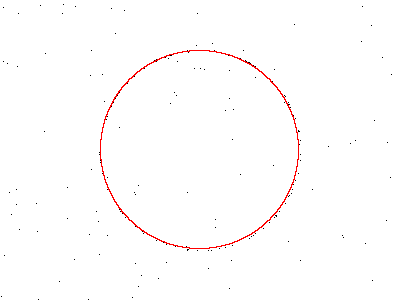
\includegraphics{circle}
\end{figure}

Analysis of the above figure leads to conclusion that the obtained circle is exactly as expected. After receiving best parameters it was drawn using function embedded in ImageJ drawOval , with these parameters.




\section {Research question A}

Given specified amount of points being total number of points, m and points which belongs to circle n, probability of drawing a 3 circle points in a random draw could be described as follows:
\[p=\frac{\binom{n}{3}}{\binom{m}{3}}\]


\section {Research question B}

The above algorithm could be somehow extended in such way that not only the best one with largest number of points in neighbourhood could be stored but a couple of them. If these circles are different then their parameters, that is center and radius should be different. The first circle with biggest number of points close to it and also with significantly different parameters can be potentially other circle. 


%%%----------------------------------------------------------
\MakeBibliography[nosplit]
%%%----------------------------------------------------------


\end{document}